\documentclass{standalone}
\usepackage{verbatim}
\usepackage{mathtools}
\usepackage{tikz}
\usetikzlibrary{positioning}
  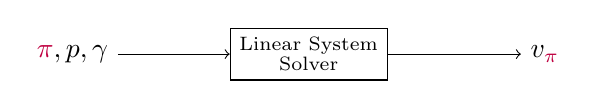
\begin{tikzpicture}
    \node (vars) at (0, 0) {$\color{purple} \pi \color{black}, p, \gamma$};
    \node[draw,rectangle] (solv) at (3, 0) {$\substack{\textrm{Linear System} \\         \textrm{Solver}}$};
    \node (vpi)  at (6, 0) {$v_{\color{purple} \pi}$};
    \draw[->] (vars) -- (solv);
    \draw[->] (solv) -- (vpi);
  \end{tikzpicture}
\end{document}